\usetikzlibrary{arrows.meta,shapes.multipart}

\begin{frame}{example: producer/consumer}
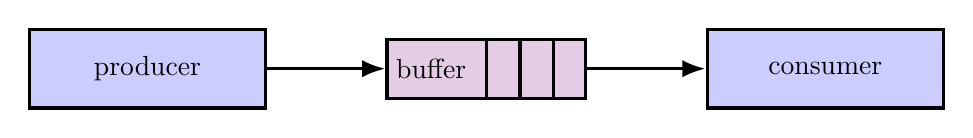
\begin{tikzpicture}
    \node[minimum width=3cm,minimum height=1cm,draw,very thick,fill=blue!20] (producer) {producer};
    \node[minimum height=0.75cm,draw,very thick,fill=violet!20,
          anchor=west,rectangle split,rectangle split horizontal,
          rectangle split parts=4] (buffer) at ([xshift=1.5cm]producer.east) {buffer
            \hspace{3cm}};
    \node[minimum width=3cm,minimum height=1cm,draw,very thick,fill=blue!20,
          anchor=west] (consumer) at ([xshift=1.5cm]buffer.east) {consumer};

    \begin{scope}[very thick,>=Latex]
        \draw[->] (producer)  -- (buffer);
        \draw[->] (buffer)  -- (consumer);
    \end{scope}
\end{tikzpicture}
    \begin{itemize}
        \item shared buffer (queue) of fixed size
            \begin{itemize}
            \item one or more producers inserts into queue
            \item one or more consumers removes from queue
            \end{itemize}
        \item<2-> producer(s) and consumer(s) don't work in lockstep
            \begin{itemize}
            \item (might need to wait for each other to catch up)
            \end{itemize}
        \item<3-> example: C compiler
            \begin{itemize}
            \item preprocessor $\rightarrow$ compiler $\rightarrow$ assembler $\rightarrow$ linker
            \end{itemize}
    \end{itemize}
\end{frame}

